\documentclass[a4paper, spanish]{article}

\usepackage[T1]{fontenc}
\usepackage[utf8]{inputenc}
\usepackage{babel, parskip}
\usepackage[colorlinks]{hyperref}
\usepackage{graphicx}


\title{Projectizer (SAR) \\ Documento de Diseño}
\author{Version 1.0 \\ M. Blanc, L.C. Jariego, P. Marcos, F. Martín, D. Nevado}

\begin{document}


\maketitle
\begin{abstract}
Este es el documento de diseño de \textit{Proyectizer}, un Sistema de Análisis de Requisitos (SAR) cuyo objetivo es servir de plataforma de gestión de requisitos para empresas de desarrollo de software.
En este documento de diseño, se concreta la implementación descrita en el documento de análisis.
\end{abstract}
\vspace{\fill}
\tableofcontents
%% Estas dos lineas son temporales
%\pagebreak
\let\oldsection\section\renewcommand\section{\clearpage\oldsection}

\section{Descripción de la Arquitectura del Sistema}
La arquitectura de este sistema informático se basa en un patrón MVC (Modelo Vista Controlador). La idea fundamental de este patrón es separar la interfaz del modelo.
 

\section{Diagrama de Clases}
\begin{figure}[h!]
\centering
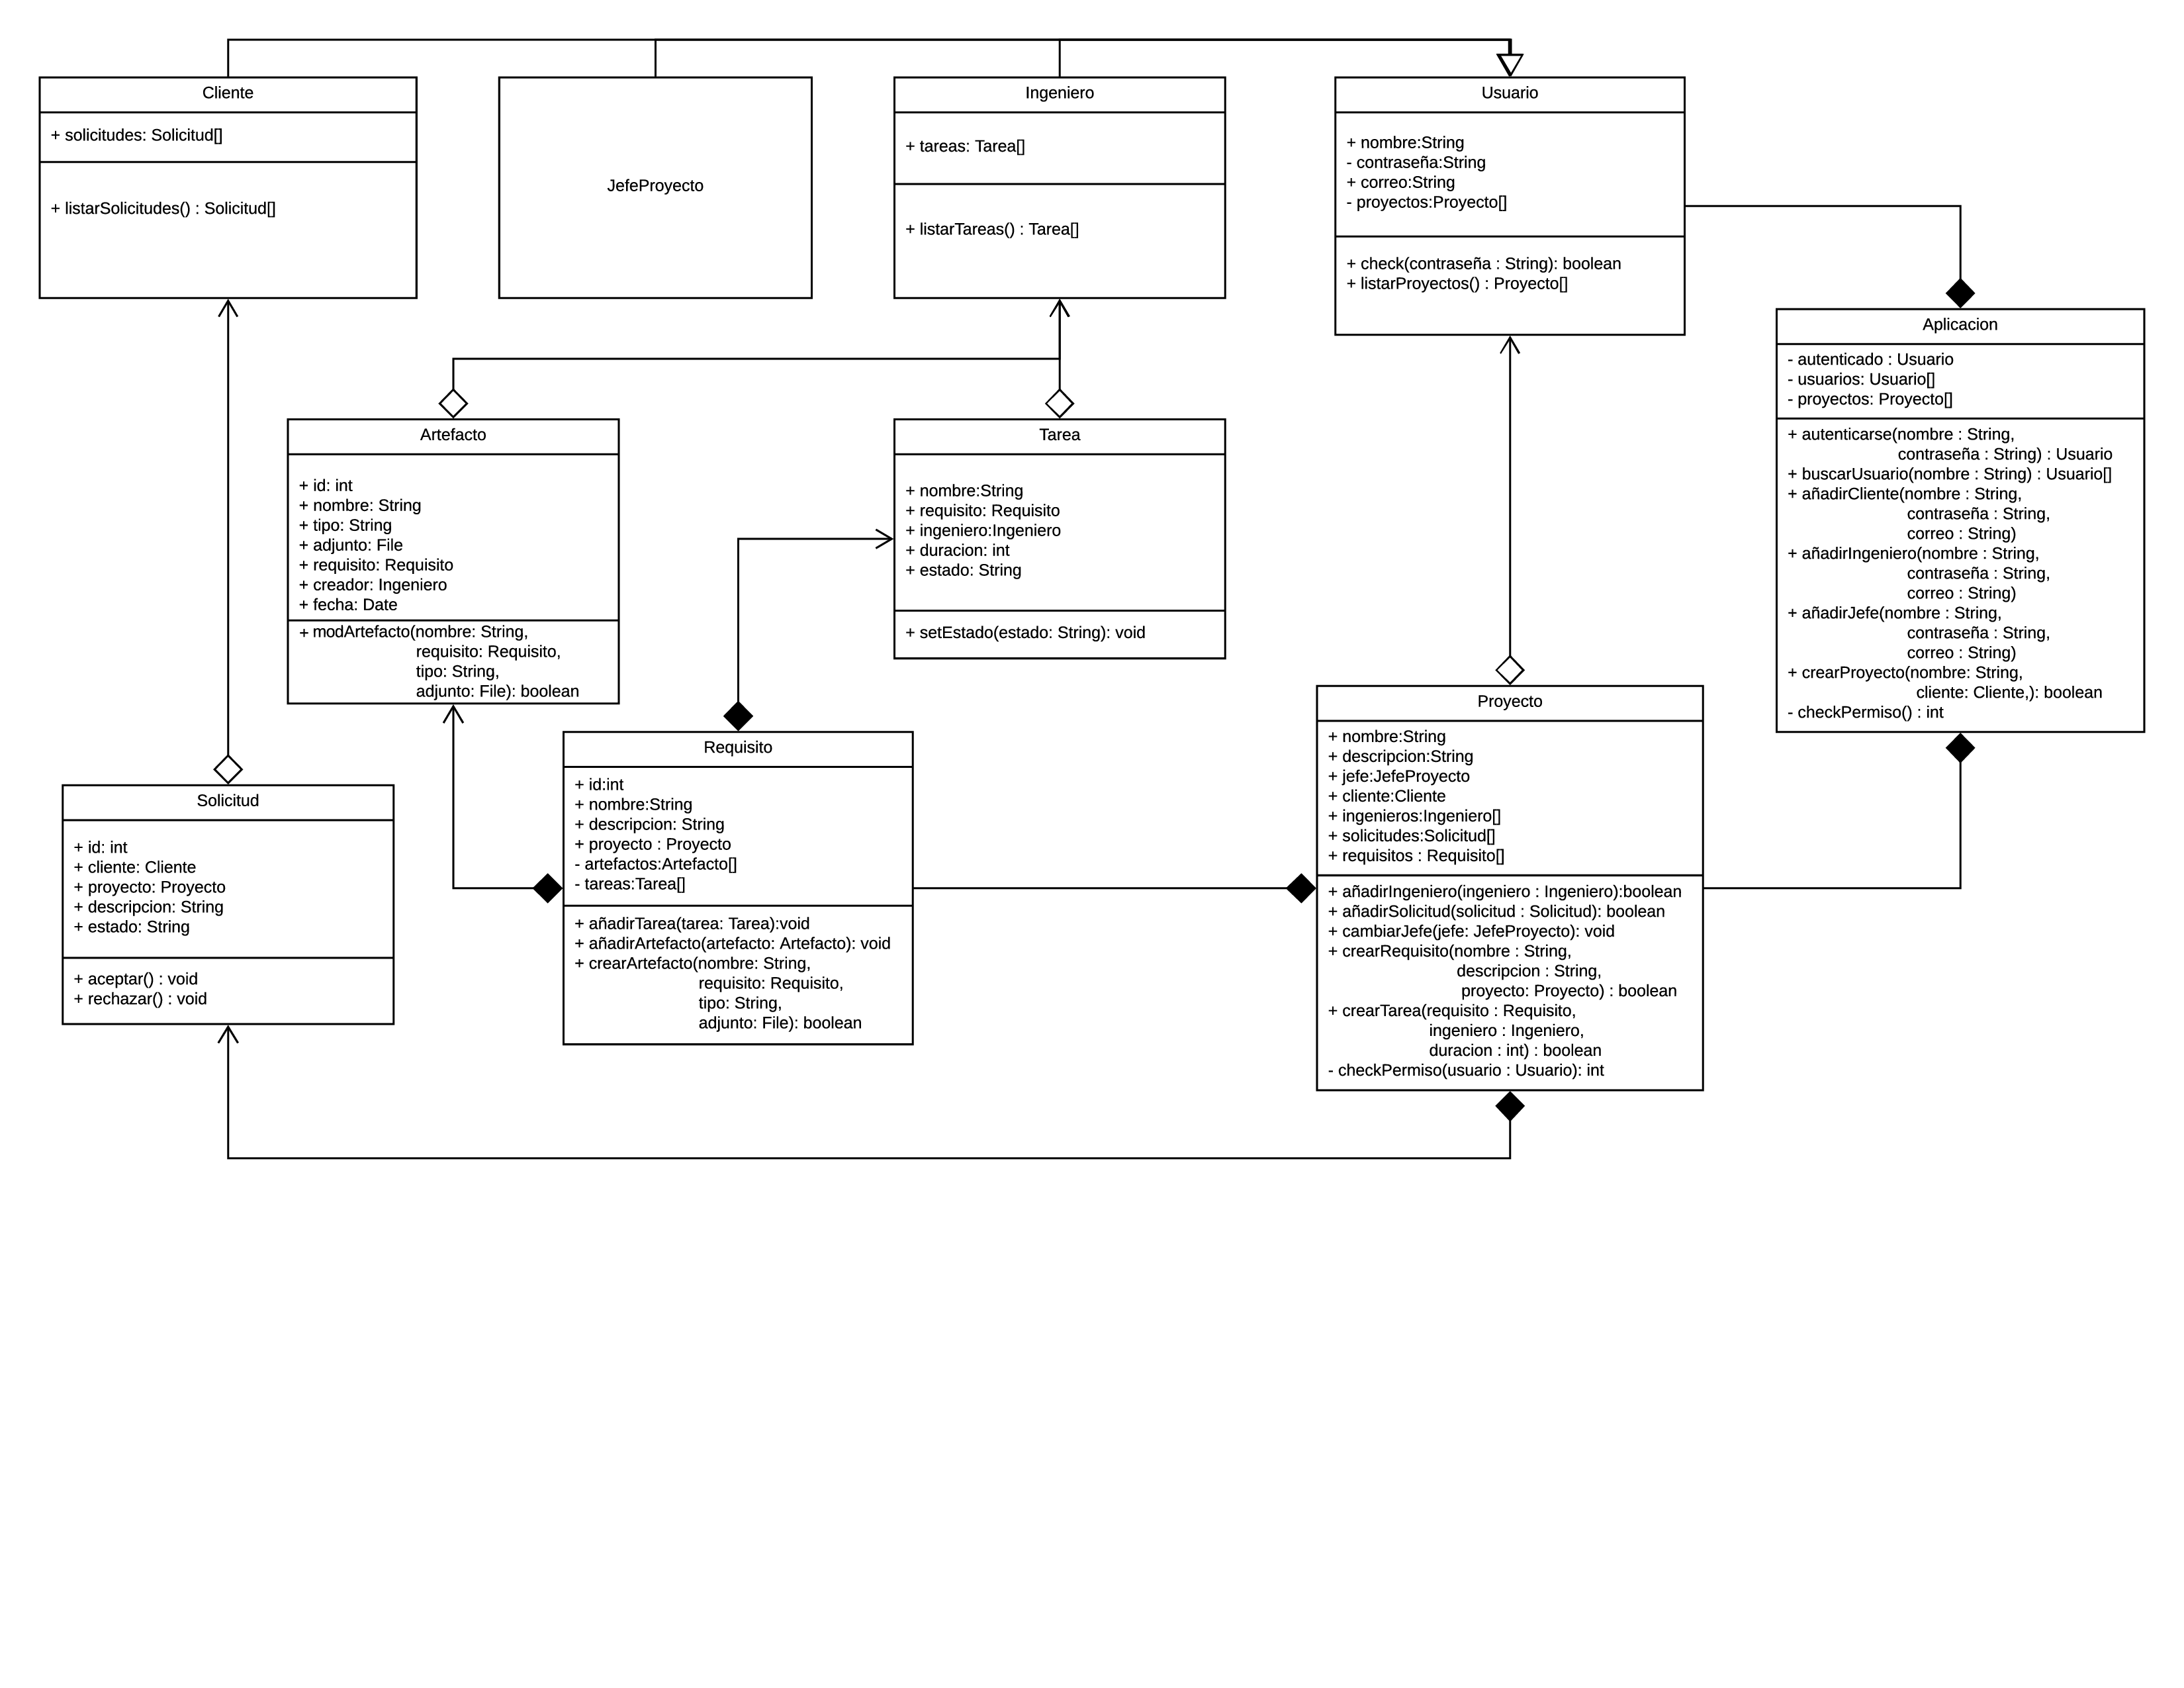
\includegraphics[width=\textwidth]{diagramas/diagrama-clases.png}
\caption{Diagrama de clases}
\end{figure}

\section{Diagramas de Secuencia}
Según UML los argumentos son opcionales.
Hemos decidido no incluirlos para no sobrecargar el diagrama y transmitir mejor el mensaje.

\pagebreak\subsection{Especificar Requisito} % Diagrama de secuencia obligatorio num 1
\begin{figure}[h!]
\centering
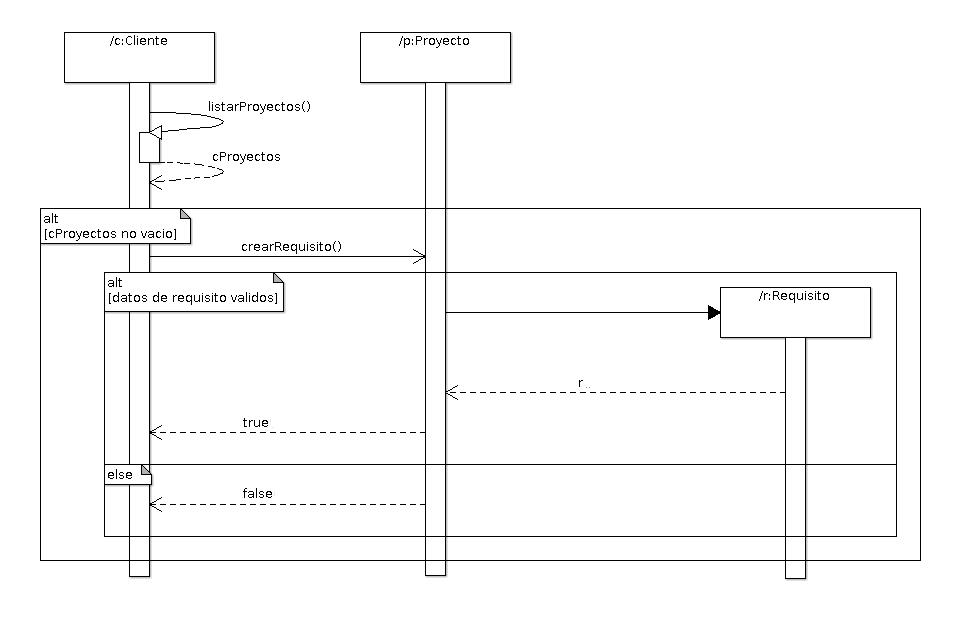
\includegraphics[width=0.9\textwidth]{diagramas/diagramasSecuencia/CrearRequisito_sd.png}
\caption{Diagrama de secuencia para CrearRequisitos}
\end{figure}
En este diagrama de flujo, el cliente obtiene la lista de proyectos para posteriormente crear los requisitos.


\pagebreak\subsection{Crear Proyecto} % Diagrama de secuencia obligatorio num 2
\begin{figure}[h!]
\centering
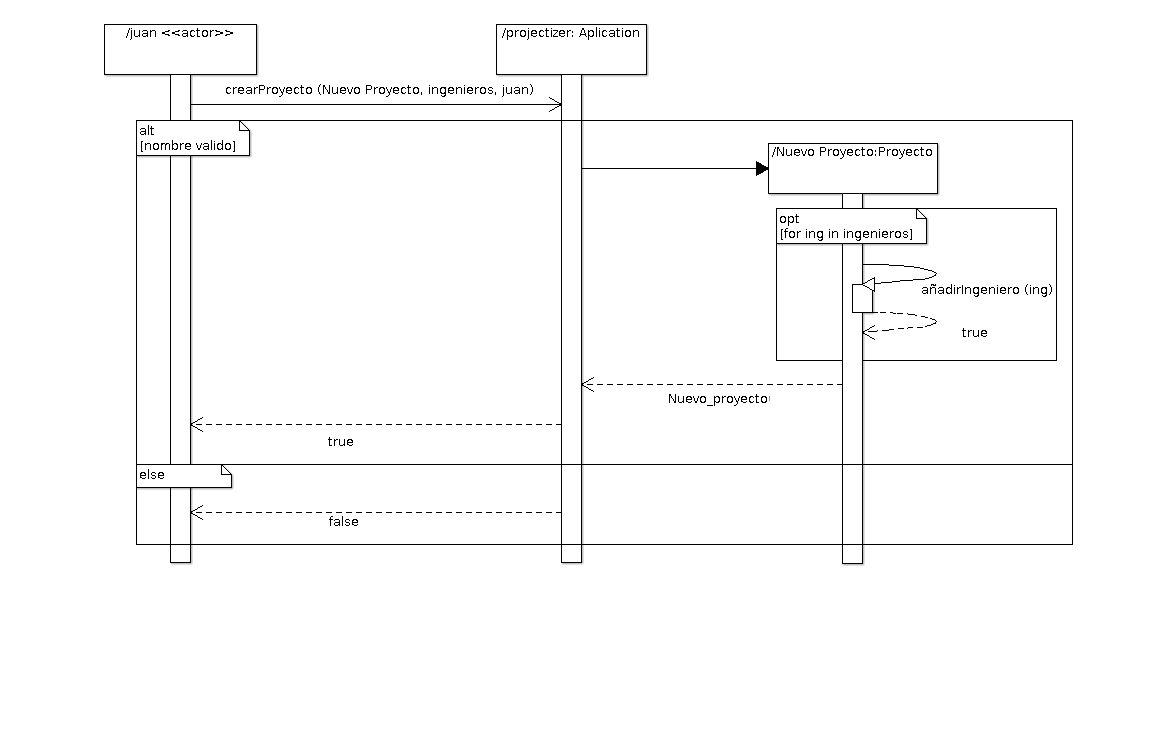
\includegraphics[width=0.9\textwidth]{diagramas/diagramasSecuencia/CrearProyecto_sd.png}
\caption{Diagrama de secuencia para CrearProyecto}
\end{figure}


\pagebreak\subsection{Crear Solicitud de Requisito} % Diagrama de secuencia obligatorio num 3
\begin{figure}[h!]
\centering
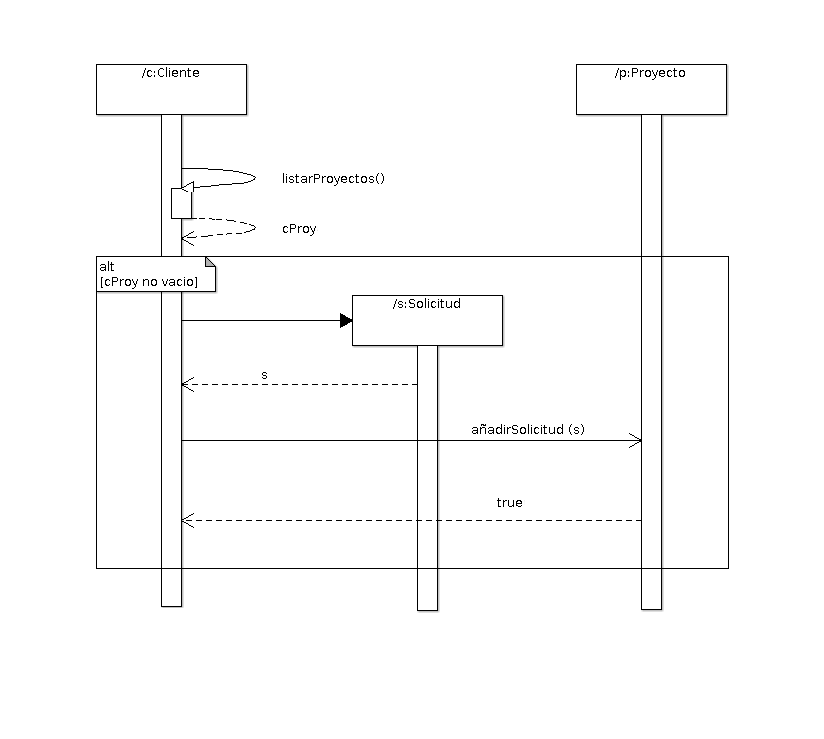
\includegraphics[width=0.9\textwidth]{diagramas/diagramasSecuencia/CrearSolicitud_sd.png}
\caption{Diagrama de secuencia para CrearSolicitud}
\end{figure}


\pagebreak\subsection{Crear Artefacto}
\begin{figure}[h!]
\centering
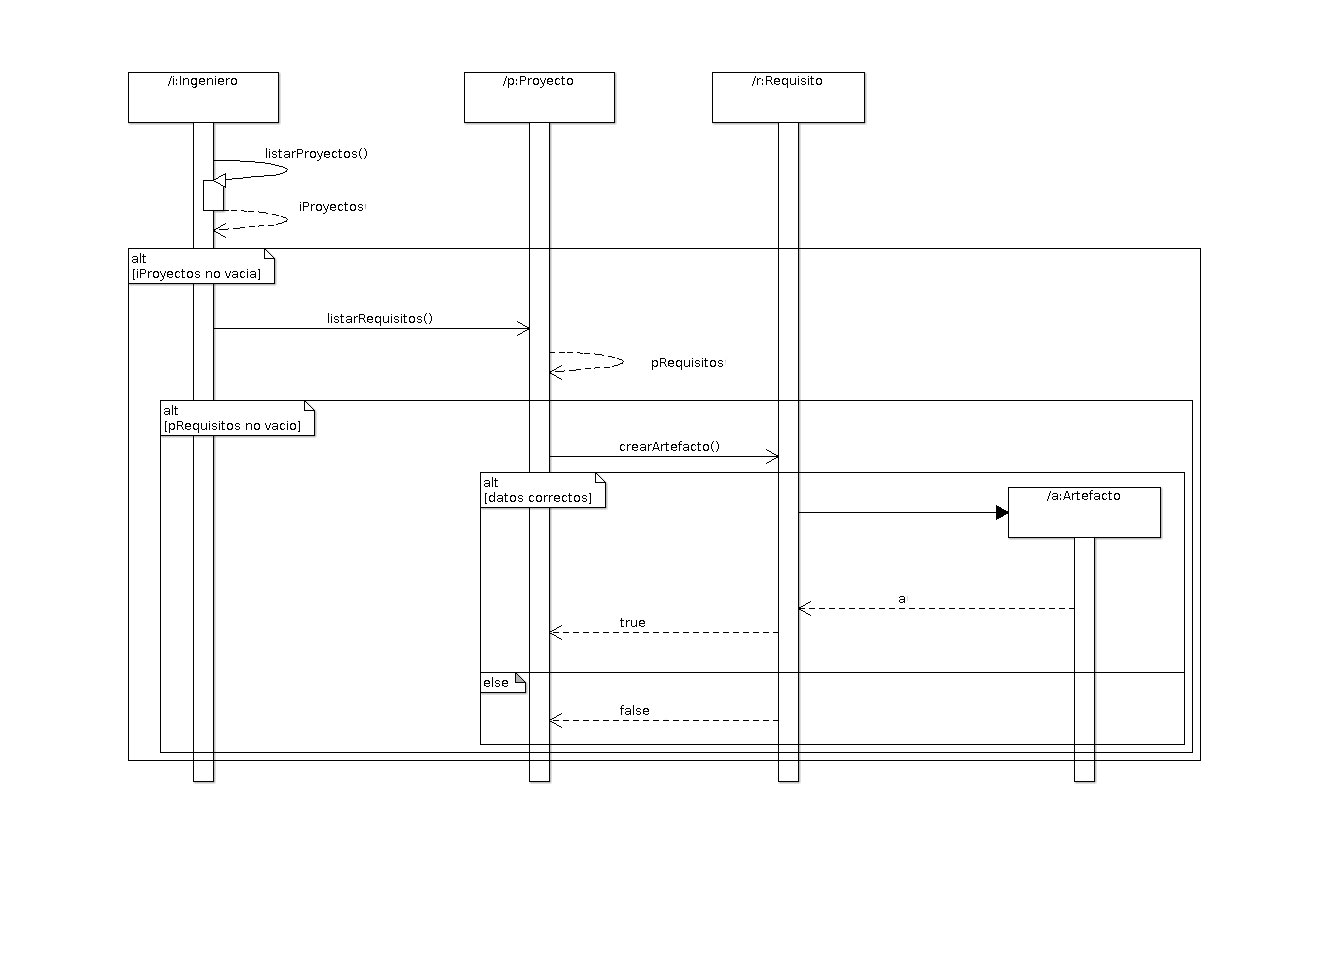
\includegraphics[width=0.9\textwidth]{diagramas/diagramasSecuencia/CrearArtefacto_sd.png}
\caption{Diagrama de secuencia para CrearArtefacto}
\end{figure}

\section{Glosario}
\begin{description}
  \item [SAR] Abreviación de Sistema de Análisis de Requisitos
  \item [JdP] Abreviación de Jefe de Proyecto
  \item [Solicitud] Solicitud de un requisito nuevo
  \item [Artefacto] Un producto tangible producido durante el desarrollo.
  \item [Scrum] Metodología de desarrollo ágil comercial. 
\end{description}

\end{document}